    % ============================================================
    %  SICOLEGIO 360 --- Documento Académico Integrado
    %  Tema: Integración ERP, Procesamiento TPS y Analítica en Power BI
    %  Curso: Sistemas de Información  |  Ciclo 7
    %  Elaborado con LaTeX (clase report) - Estilo APA 7
    % ============================================================
    \documentclass[12pt,a4paper,oneside]{report}

    % -- Paquetes esenciales -------------------------------------
    \usepackage[T1]{fontenc}
    \usepackage[utf8]{inputenc}
    \usepackage[provide=*,spanish]{babel}
    \addto\captionsspanish{\renewcommand{\tablename}{Tabla}}
    \addto\captionsspanish{\renewcommand{\listtablename}{\'Indice de Tablas}}
    \addto\captionsspanish{\renewcommand{\listfigurename}{\'Indice de Figuras}}
    \addto\captionsspanish{\renewcommand{\appendixname}{Anexo}}
    \addto\captionsspanish{\renewcommand{\contentsname}{\'Indice General}}
    \usepackage{lmodern}

    % -- Geometría -----------------------------------------------
    \usepackage[
    top=2.54cm, bottom=2.54cm,
    left=2.54cm, right=2.54cm,
    headheight=28pt
    ]{geometry}

    % -- Colores -------------------------------------------------
    \usepackage[table]{xcolor}
    \definecolor{azulOscuro}{RGB}{10,47,97}
    \definecolor{azulMedio}{RGB}{28,100,180}
    \definecolor{verdInst}{RGB}{34,120,80}
    \definecolor{grisClaro}{RGB}{245,246,248}
    \definecolor{grisTabla}{RGB}{220,225,232}
    \definecolor{dorado}{RGB}{180,140,20}

    % -- Tipografía (Times New Roman para APA 7) -----------------
    \usepackage{times}

    % -- Encabezados y pies (Formato APA 7 sin colores ni líneas) -
    \usepackage{fancyhdr}
    \pagestyle{fancy}
    \fancyhf{}
    \fancyhead[L]{\small\MakeUppercase{SICOLEGIO 360: ERP Educativo \& Analítica Power BI}}
    \fancyhead[R]{\thepage}
    \fancyfoot{}
    \renewcommand{\headrulewidth}{0pt}

    % -- Secciones en formato APA 7 ------------------------------
    \usepackage{titlesec}
    \titleformat{\chapter}
    {\normalfont\bfseries\Large\centering}
    {\thechapter\quad}
    {0pt}
    {}
    \titlespacing*{\chapter}{0pt}{-25pt}{15pt}
    \titleformat{\section}
    {\normalfont\bfseries\large}{\thesection}{1em}{}
    \titleformat{\subsection}
    {\normalfont\bfseries\itshape\normalsize}{\thesubsection}{1em}{}
    \titleformat{\subsubsection}
    {\normalfont\bfseries\normalsize}{\thesubsubsection}{1em}{}

    % -- Listas --------------------------------------------------
    \usepackage{enumitem}
    \setlist[itemize]{leftmargin=1.5em,itemsep=2pt,topsep=4pt}
    \setlist[enumerate]{leftmargin=1.5em,itemsep=2pt,topsep=4pt}

    % -- Tablas --------------------------------------------------
    \usepackage{booktabs}
    \usepackage{longtable}
    \usepackage{array}
    \usepackage{multirow}
    \usepackage{tabularx}
    \usepackage{xltabular}
    \renewcommand{\arraystretch}{1.35}

    % -- Figuras y Captions al estilo APA 7 ----------------------
    \usepackage{graphicx}
    \usepackage{float}
    \usepackage{caption}
    \usepackage{subcaption}
    \captionsetup[table]{labelfont=bf,textfont=it,labelsep=newline,singlelinecheck=off,justification=raggedright}
    \captionsetup[figure]{labelfont=bf,textfont=it,labelsep=newline,singlelinecheck=off,justification=raggedright}

    % -- Hiperenlaces --------------------------------------------
    \usepackage{hyperref}
    \hypersetup{
    colorlinks=true,
    linkcolor=black,
    citecolor=black,
    urlcolor=black,
    pdftitle={SICOLEGIO 360 — ERP Educativo, TPS y Analítica Power BI},
    pdfauthor={Curso Sistemas de Información},
    pdfsubject={Proyecto académico de integración transaccional y analítica gerencial},
    }

    % -- Bibliografía APA 7 --------------------------------------
    \usepackage[authoryear]{natbib}
    \setcitestyle{authoryear,round,aysep={,}}

    % -- Utilidades ----------------------------------------------
    \usepackage{amsmath}
    \usepackage{amssymb}
    \usepackage{tocloft}
    \setcounter{tocdepth}{2}
    \renewcommand{\cfttoctitlefont}{\hfill\normalfont\bfseries\Large}
    \renewcommand{\cftaftertoctitle}{\hfill}
    \renewcommand{\cftlottitlefont}{\hfill\normalfont\bfseries\Large}
    \renewcommand{\cftafterlottitle}{\hfill}
    \renewcommand{\cftloftitlefont}{\hfill\normalfont\bfseries\Large}
    \renewcommand{\cftafterloftitle}{\hfill}
    \renewcommand{\cftchapleader}{\cftdotfill{\cftdotsep}}
    \setlength{\cftbeforetoctitleskip}{-25pt}
    \setlength{\cftaftertoctitleskip}{15pt}
    \setlength{\cftbeforelottitleskip}{-25pt}
    \setlength{\cftafterlottitleskip}{15pt}
    \setlength{\cftbeforeloftitleskip}{-25pt}
    \setlength{\cftafterloftitleskip}{15pt}
    \usepackage{rotating}
    \usepackage{framed}
    \usepackage{setspace}
    \usepackage{listings}
    \usepackage{xcolor}

    \lstset{
        basicstyle=\ttfamily\small,
        breaklines=true,
        breakatwhitespace=true,
        frame=single,
        columns=fullflexible,
        keepspaces=true,
        keywordstyle=\bfseries\color{blue},
        commentstyle=\itshape\color{gray},
        stringstyle=\color{teal}
    }

    % -- Espaciado y Sangrías APA 7 -----------------------------
    \usepackage{indentfirst}
    \setlength{\parskip}{0pt}
    \setlength{\parindent}{1.27cm}

    % -- Caja destacada ------------------------------------------
    \newenvironment{cajaConcepto}[1][]{%
    \begin{framed}\noindent{\bfseries #1}\par\smallskip
    }{\end{framed}}

    % ═══════════════════════════════════════════════════════════════
    \begin{document}
    \sloppy
    \doublespacing

    % ─────────────────────────────────────────────────────────────
    %  PORTADA (Estilo APA 7 - Sobrio)
    % ─────────────────────────────────────────────────────────────
    \begin{titlepage}
        \begin{center}
            \setstretch{1.1}
            {\fontsize{14}{16}\selectfont\textbf{UNIVERSIDAD NACIONAL AGRARIA DE LA SELVA}} \\[0.3cm]
            {\fontsize{13}{15}\selectfont\textbf{FACULTAD DE INGENIERÍA EN INFORMÁTICA Y SISTEMAS}} \\[0.2cm]
            {\fontsize{12}{14}\selectfont\textbf{ESCUELA PROFESIONAL DE INGENIERÍA DE SISTEMAS}} \\[0.4cm]
            
            \begin{minipage}{0.45\textwidth}
                \centering
                \includegraphics[height=7.5cm,keepaspectratio]{logounas.png}
            \end{minipage}
            \hfill
            \begin{minipage}{0.45\textwidth}
                \centering
                \includegraphics[height=4.8cm,keepaspectratio]{LOGO-FIIS-1000x1000-TR.png}
            \end{minipage}\\[0 cm]
            
            \rule{\linewidth}{1.5pt} \\[0.6cm]
            
            {\fontsize{13}{16}\selectfont\textbf{INTEGRACIÓN DE SISTEMAS DE INFORMACIÓN, PROCESAMIENTO DE TRANSACCIONES TPS Y ANALÍTICA DE NEGOCIOS EN POWER BI: ANÁLISIS DE LA INTERACCIÓN ENTRE LA DIRECCIÓN ACADÉMICA Y EL CONTROL ESCOLAR EN SICOLEGIO 360}} \\[0.6cm]
            
            \rule{\linewidth}{1.5pt} \\[1.2cm]
            
            \setstretch{1.5}
            \begin{minipage}{0.85\textwidth}
                \begin{flushleft}
                    \begin{tabular}{@{}p{3.5cm}p{9.5cm}@{}}
                        \textbf{Curso:} & Sistemas de Información \\[0.2cm]
                        \textbf{Autores:} & Evaristo Jara, Jose Junior \\
                                        & Tapullima Serna, Meselemias \\[0.2cm]
                        \textbf{Docente:} & Docente del Curso \\[0.2cm]
                        \textbf{Ciclo:} & Séptimo \\[0.2cm]
                    \end{tabular}
                \end{flushleft}
            \end{minipage}
            
            \vfill
            
            {\fontsize{12}{14}\selectfont\textbf{Tingo María -- Perú}} \\[0.2cm]
            {\fontsize{12}{14}\selectfont\textbf{2026}}
        \end{center}
    \end{titlepage}

    % ─────────────────────────────────────────────────────────────
    %  RESUMEN
    % ─────────────────────────────────────────────────────────────
    \chapter*{Resumen}
    \addcontentsline{toc}{chapter}{Resumen}
    \markboth{RESUMEN}{RESUMEN}

    El presente estudio académico aborda el diseño, integración e ingeniería analítica de \textbf{SICOLEGIO 360}, concebido como una plataforma de gestión para el sector educativo sustentada sobre una arquitectura de sistemas transaccionales desacoplados e integración en Business Intelligence. Frente al diagnóstico de desarticulación operativa en instituciones educativas —caracterizadas por la falta de sincronización entre el rendimiento pedagógico del aula y el control de asistencia y disciplina de los alumnos—, este documento demuestra el valor de acoplar operativamente dos Sistemas de Procesamiento de Transacciones (\textbf{TPS}): el \textbf{TPS Pedagógico} (Dirección Académica) y el \textbf{TPS de Control Escolar y Convivencia} (Secretaría/Auxiliaría).

    El trabajo profundiza en la interacción transaccional entre ambas áreas: la \textbf{Dirección Académica} (encargada del registro de evaluaciones, notas, promedios bimestrales, libretas y horarios) y la \textbf{Secretaría Escolar y Convivencia} (encargada de la admisión, matrículas, marcación diaria de asistencia, justificaciones, registro disciplinario y citaciones). Se analiza el flujo de datos garantizando las propiedades ACID mediante transacciones SQL y disparadores que automatizan la justificación de evaluaciones y las alertas por desaprobación o inasistencias acumuladas.

    Asimismo, la investigación diferencia explícitamente los reportes operativos en tiempo real integrados en el código de la aplicación web de SICOLEGIO 360 (\textbf{MIS}) de la capa de Business Intelligence desarrollada en \textbf{Power BI} (\textbf{DSS/BI}). En esta última se establece la arquitectura ETL, el modelado dimensional en estrella (\textit{Star Schema}), la creación de medidas en lenguaje DAX (tasa de asistencia ponderada, porcentaje de desaprobación, índice de incidencias y correlación asistencia-rendimiento) y la aplicación de políticas de seguridad a nivel de fila (\textit{Row-Level Security - RLS}). Finalmente, se consolida una matriz de toma de decisiones que conecta los indicadores operativos con la planificación estratégica del colegio.

    \textbf{Palabras clave:} Sistemas de Información, TPS Pedagógico, TPS Control Escolar, Desacoplamiento Transaccional, Propiedades ACID, Dirección Académica, Convivencia Escolar, Power BI, Modelo en Estrella, DAX, Row-Level Security, MIS, DSS.

    % ─────────────────────────────────────────────────────────────
    %  ABSTRACT
    % ─────────────────────────────────────────────────────────────
    \chapter*{Abstract}
    \addcontentsline{toc}{chapter}{Abstract}
    \markboth{ABSTRACT}{ABSTRACT}

    This academic research addresses the design, integration, and analytical engineering of \textbf{SICOLEGIO 360}, conceived as an educational management platform backed by a decoupled Transaction Processing System architecture integrated with Business Intelligence. Based on the diagnosis of operational fragmentation in schools —characterized by unaligned data between classroom pedagogical performance and daily attendance and behavioral control— this paper demonstrates the value of coupling two Transaction Processing Systems (\textbf{TPS}): the \textbf{Pedagogical TPS} (Academic Directorate) and the \textbf{School Control & Coexistence TPS} (Secretariat/Discipline Office).

    The paper delves into the transactional interaction between both departments: \textbf{Academic Directorate} (responsible for evaluation records, grades, bimonthly averages, report cards, and schedules) and \textbf{School Control & Coexistence} (in charge of admissions, enrollments, daily attendance tracking, absence justifications, behavioral records, and parent summons). The data flow is analyzed while guaranteeing ACID properties through SQL transactions and triggers that automate assessment rescheduling and alerts for cumulative absences or academic failure.

    Furthermore, this study explicitly differentiates real-time operational reporting embedded within the SICOLEGIO 360 web application codebase (\textbf{MIS}) from the Business Intelligence layer engineered in \textbf{Power BI} (\textbf{DSS/BI}). The latter establishes ETL architecture, Star Schema dimensional modeling, DAX measure calculations (weighted attendance rate, failure percentage, disciplinary incident index, and attendance-performance correlation), and Row-Level Security (RLS) policies for multi-tenant data governance. Finally, a decision-making matrix is consolidated to bridge operational indicators with executive institutional planning.

    \textbf{Keywords:} Information Systems, Pedagogical TPS, School Control TPS, Transactional Decoupling, ACID Properties, Academic Management, School Coexistence, Power BI, Star Schema, DAX, Row-Level Security, MIS, DSS.

    % ─────────────────────────────────────────────────────────────
    %  ÍNDICES
    % ─────────────────────────────────────────────────────────────
    \newpage 
    \tableofcontents
    \newpage
    \listoftables
    \newpage
    \listoffigures

    % ─────────────────────────────────────────────────────────────
    %  INTRODUCCIÓN
    % ─────────────────────────────────────────────────────────────
    \chapter*{Introducción}
    \addcontentsline{toc}{chapter}{Introducción}
    \markboth{INTRODUCCIÓN}{INTRODUCCIÓN}

    En el sector educativo privado de nivel básico regular en el Perú y América Latina, la eficiencia institucional depende críticamente de la capacidad de sincronizar los flujos académicos con la sostenibilidad financiera. Históricamente, las instituciones educativas privadas de tamaño pequeño y mediano han operado bajo esquemas fragmentados: la Secretaría Académica gestiona las fichas de los estudiantes y el control de aula en cuadernos de notas o archivos locales de Excel, mientras que la Tesorería maneja la cobranza de pensiones en comprobantes físicos o software contable no acoplado.

    Esta desarticulación genera graves "islas de información". La consecuencia inmediata es la aparición de cuellos de botella operativos: alumnos matriculados sin la validación de compromisos financieros, sobreaforo en aulas por falta de control en tiempo real, morosidad detectada tardíamente al cierre del año lectivo y la imposibilidad de la alta dirección para tomar decisiones estratégicas basadas en evidencia cuantitativa confiable.

    El presente trabajo de investigación académica presenta una solución integral estructurada en la plataforma \textbf{SICOLEGIO 360}. El proyecto demuestra cómo un \textbf{ERP Educativo (Ed-ERP)}, sustentado en una \textbf{base de datos relacional centralizada}, actúa como la única fuente de verdad (\textit{Single Source of Truth - SSOT}) de la institución. Sobre este núcleo se ejecutan las transacciones operativas diarias (\textbf{TPS}) garantizando la rigurosidad de las propiedades ACID (Atomicidad, Consistencia, Aislamiento y Durabilidad).

    El documento se estructura en seis capítulos sistemáticos: el \textbf{Capítulo I} desarrolla el marco conceptual de los Ed-ERP y la base de datos centralizada; el \textbf{Capítulo II} detalla la ingeniería transaccional y los flujos BPMN entre Secretaría y Tesorería; el \textbf{Capítulo III} diseña la capa de métricas, KPIs y requerimientos de información por rol; el \textbf{Capítulo IV} expone la reportería operativa nativa en el software web (MIS); el \textbf{Capítulo V} fundamenta la arquitectura analítica avanzada en Power BI (DSS/BI); y el \textbf{Capítulo VI} consolida la matriz de toma de decisiones y el plan de mejora continua, finalizando con las conclusiones, recomendaciones y referencias bibliográficas en formato APA 7.

    % ═══════════════════════════════════════════════════════════════
    %  CAPÍTULO I: ARQUITECTURA ERP Y BASE DE DATOS CENTRALIZADA
    % ═══════════════════════════════════════════════════════════════
    \chapter{Marco Conceptual: Arquitectura ERP y Base de Datos Centralizada en SICOLEGIO 360}

    \section{Evolución Histórica y Justificación Socio-Tecnológica del Ed-ERP}

    La gestión de la información en las instituciones educativas privadas de nivel básico regular en el Perú y América Latina ha atravesado una evolución caracterizada por tres etapas históricas marcadas por el nivel de madurez tecnológica:

    \begin{enumerate}
        \item \textbf{Era de los Registros Manuales (Antes de 1995):} La administración escolar dependía exclusivamente de archivos físicos, libretas de papel, carpetas colgantes y libros contables manuscritos. La velocidad de procesamiento era extremadamente lenta, la búsqueda de antecedentes tomaba días y el riesgo de pérdida o deterioro físico por causas ambientales o humanas era muy elevado.
        \item \textbf{Era de la Ofimática Desconectada (1995 - 2015):} Con la masificación de los computadores personales, los colegios migraron sus archivos a procesadores de texto y hojas de cálculo locales (Excel). Si bien este paso aceleró la mecanización del trabajo, introdujo el fenómeno de las \textit{"islas de información"}. Cada departamento (Secretaría, Tesorería, Docencia) mantenía sus propios archivos de Excel en computadores independientes, generando múltiples versiones contradictorias del mismo estudiante, duplicidad de digitación y frecuentes descuadres de caja.
        \item \textbf{Era de los Sistemas de Planificación de Recursos Empresariales Educativos (Ed-ERP) (2015 en adelante):} Frente a la complejidad operativa actual, surge la necesidad de adoptar la filosofía de Planificación de Recursos Empresariales (ERP, por sus siglas en inglés \textit{Enterprise Resource Planning}) adaptada al entorno escolar. Un \textbf{Ed-ERP} se define como una suite de software modular integradora que automatiza y coordina la totalidad de las actividades académicas, administrativas, financieras y pedagógicas de la institución a través de una arquitectura de software unificada y un repositorio de datos común \citep{laudon2016}.
    \end{enumerate}

    SICOLEGIO 360 se fundamenta en el \textbf{Enfoque Socio-Tecnológico}, el cual sostiene que el rendimiento de un sistema de información no depende únicamente de la sofisticación técnica del software o hardware, sino del ajuste armónico entre la dimensión técnica (base de datos relacional, pasarelas de pago, servidores web) y la dimensión social (personal administrativo, plana docente, equipo directivo, estudiantes y apoderados). La introducción de SICOLEGIO 360 no busca imponer herramientas complejas, sino aplanar la estructura jerárquica escolar, descentralizar la entrada de datos en la fuente y automatizar las tareas repetitivas para que el personal se enfoque en la calidad educativa y la atención humana.

    \section{Estructura Jerárquica del Sistema SICOLEGIO 360 y Delimitación del Alcance}

La institución educativa opera bajo una estructura organizacional integral que articula la gestión estratégica, administrativa y pedagógica. La Figura~\ref{fig:estructura_jerarquica} describe el organigrama general de la institución:

\begin{figure}[H]
    \centering
    \begin{cajaConcepto}[Estructura Jerárquica e Institucional del Colegio]
    \textbf{1. Dirección y Promotoría (Nivel Superior):}
    \begin{itemize}
        \item \textit{Órgano Promotor y Directorio:} Define las políticas institucionales y de inversión.
        \item \textit{Dirección General / Director:} Supervisa el cumplimiento de metas y gestiona la analítica estratégica en Power BI.
        \item \textit{Área de Sistemas, Datos y Análisis SICOLEGIO 360:} Soporte técnico y gestión de la plataforma.
    \end{itemize}

    \textbf{2. Staff de Gestión y Control (Nivel Soporte):}
    \begin{itemize}
        \item Secretaría General, Administración y Tesorería, Consejo Directivo y Asesoría Contable.
    \end{itemize}

    \textbf{3. Subdirección Académica (Área 1 -- Alcance TPS Pedagógico):}
    \begin{itemize}
        \item Coordinación de los Niveles Inicial, Primaria y Secundaria, y el Cuerpo Docente de aula.
    \end{itemize}

    \textbf{4. Subdirección de Formación y Convivencia (Área 2 -- Alcance TPS Control Escolar):}
    \begin{itemize}
        \item Departamento Psicopedagógico, Tutoría, Convivencia Escolar, Auxiliares de Educación y Consejo Escolar.
    \end{itemize}

    \textbf{5. Comunidad Escolar e Interacción Externa:}
    \begin{itemize}
        \item Estudiantes y Padres de Familia / Apoderados.
    \end{itemize}
    \end{cajaConcepto}
    \caption{Estructura jerárquica organizacional de la institución educativa SICOLEGIO 360}
    \label{fig:estructura_jerarquica}
\end{figure}

\paragraph{Delimitación del Alcance Técnico del Proyecto:}
Si bien el organigrama representa la totalidad de las dependencias institucionales, la presente investigación delimita formalmente su alcance técnico al análisis del procesamiento transaccional (\textbf{TPS}) e interacción interdepartamental entre dos áreas clave:
\begin{enumerate}
    \item \textbf{Subdirección Académica (Área 1):} Responsable de la gestión del \textbf{TPS Pedagógico y Evaluativo} (\texttt{notas}, \texttt{evaluaciones}, \texttt{promedios}, \texttt{horarios}).
    \item \textbf{Subdirección de Formación y Convivencia (Área 2):} Responsable de la gestión del \textbf{TPS de Control Escolar} (\texttt{matriculas}, \texttt{asistencias}, \texttt{justificaciones}, \texttt{conducta}, \texttt{citaciones}).
\end{enumerate}

\section{Mapeo de la Pirámide Organizacional Escolar (Modelo de Laudon \& Laudon)}

    Para comprender la articulación de SICOLEGIO 360 dentro de la estructura jerárquica de una institución educativa, el sistema proyecta sus funciones a lo largo de los cuatro niveles tradicionales de la pirámide organizacional descrita por \citet{laudon2016}:

    \begin{figure}[H]
        \centering
        \begin{cajaConcepto}[Mapeo de Sistemas de Información en la Pirámide Escolar]
        \textbf{1. Nivel Estratégico (Dirección General / Promotora):}
        \begin{itemize}
            \item \textit{Sistema Evaluado:} Executive Support Systems (ESS) / Decision Support Systems (DSS) en Power BI.
            \item \textit{Función:} Análisis de proyecciones de recaudación (ARR), retención estudiantil e inversión institucional.
        \end{itemize}
        \textbf{2. Nivel Táctico / Administrativo (Administración / Dirección Académica):}
        \begin{itemize}
            \item \textit{Sistema Evaluado:} Management Information Systems (MIS) / Dashboards Web Nativos.
            \item \textit{Función:} Monitoreo diario del aforo de aulas, cuadre de caja, avance del sílabo y control de mora.
        \end{itemize}
        \textbf{3. Nivel de Conocimiento (Plana Docente / Psicopedagogía):}
        \begin{itemize}
            \item \textit{Sistema Evaluado:} Knowledge Work Systems (KWS) / Módulo de Evaluación por Competencias.
            \item \textit{Función:} Registro de calificaciones CNEB, diseño de unidades didácticas y bitácora psicopedagógica.
        \end{itemize}
        \textbf{4. Nivel Operativo (Secretaría Académica / Tesorería / Cajeros):}
        \begin{itemize}
            \item \textit{Sistema Evaluado:} Transaction Processing Systems (TPS).
            \item \textit{Función:} Ejecución masiva de transacciones atómicas (matricular alumno, cobrar pensión, emitir recibo).
        \end{itemize}
        \end{cajaConcepto}
        \caption{Mapeo funcional de SICOLEGIO 360 en la pirámide organizacional escolar}
        \label{fig:piramide_organizacional}
    \end{figure}

    Esta visión piramidal demuestra cómo los datos recopilados en el nivel operativo básico (TPS) por secretarios y tesoreros fluyen hacia arriba de forma sintetizada hacia los reportes tácticos (MIS) y finalmente alimentan los dashboards analíticos avanzados (DSS/BI) utilizados por los dueños y directores del colegio.

    \section{La Base de Datos Relacional Centralizada como Única Fuente de Verdad (SSOT)}

    El núcleo ingenieril que sustenta la propuesta de SICOLEGIO 360 es su **base de datos relacional centralizada**. En las organizaciones escolares no integradas, la fragmentación de repositorios locales conduce a la presencia de datos incongruentes. El principio de la **Única Fuente de Verdad** (\textit{Single Source of Truth - SSOT}) establece que cada entidad de información del colegio (estudiante, apoderado, sección, pensión) debe almacenarse en un único lugar lógico dentro de la base de datos relacional.

    Para lograr este objetivo sin generar vulnerabilidades de integridad, la arquitectura de datos de SICOLEGIO 360 se rige por tres pilares teóricos:

    \begin{enumerate}
        \item \textbf{Normalización Relacional Estricta (Tercera Forma Normal - 3FN):} El diseño relacional se encuentra estructurado bajo las reglas de normalización enunciadas por \citet{date2004}. Esto elimina las redundancias de datos y previene las anomalías de inserción, actualización y borrado. Por ejemplo, la información personal de un apoderado se almacena en la tabla \texttt{apoderados} de forma única, aunque dicho apoderado tenga tres hijos matriculados en distintos grados.
        \item \textbf{Arquitectura Multi-Tenant (Multiinstitucional):} Como plataforma SaaS, SICOLEGIO 360 gestiona múltiples colegios desde una sola infraestructura relacional. La privacidad y el aislamiento de datos se garantizan mediante discriminadores lógicos institucionales (\texttt{id\_colegio}) en cada tabla, respaldados por políticas de seguridad RLS (\textit{Row-Level Security}).
        \item \textbf{Gobierno de Datos y Trazabilidad (RBAC):} El control de acceso basado en roles (\textit{Role-Based Access Control}) restringe las operaciones de lectura y escritura según el perfil del usuario autenticado (Secretario, Tesorero, Docente, Padre). Todas las transacciones modificatorias registran metadatos de auditoría (usuario, marca de tiempo \texttt{TIMESTAMP}, dirección IP).
    \end{enumerate}

    \section{Catálogo Detallado de Módulos Funcionales y Reglas de Negocio}

    La Plataforma SICOLEGIO 360 articula las operaciones de la institución a través de seis módulos funcionales especializados que interactúan dinámicamente. La Tabla~\ref{tab:modulos_erp} presenta el catálogo modular completo con sus actores y responsabilidades.

    \begin{xltabular}{\textwidth}{|p{3.8cm}|X|p{4.2cm}|}
    \caption{Módulos funcionales y distribución por TPS en SICOLEGIO 360} \label{tab:modulos_erp} \\
    \hline
    \textbf{Módulo del Sistema} & \textbf{Función Principal y TPS Asignado} & \textbf{Actores Involucrados} \\
    \hline
    \endfirsthead

    \multicolumn{3}{c}{{\bfseries Tabla \thetable{} -- Continuación de la página anterior}} \\
    \hline
    \textbf{Módulo del Sistema} & \textbf{Función Principal y TPS Asignado} & \textbf{Actores Involucrados} \\
    \hline
    \endhead

    \hline
    \multicolumn{3}{r}{\textit{Continúa en la siguiente página...}} \\
    \endfoot

    \hline
    \endlastfoot

    \textbf{Dirección Académica y Evaluación} & **TPS 1 (Pedagógico):** Carga de notas por competencias, evaluaciones bimestrales, promedios y generación de libretas escolares. & Coordinador Académico, Docentes de asignatura. \\
    \hline
    \textbf{Gestión Curricular y Horarios} & **TPS 1 (Pedagógico):** Malla curricular, asignación de cursos por grado, secciones y bloques de horarios docentes. & Jefe de Estudios, Profesores. \\
    \hline
    \textbf{Secretaría y Matrícula} & **TPS 2 (Control Escolar):** Registro de admisión, expedientes de estudiantes, asignación de aforo y matrículas. & Secretario Académico, Auxiliar de Secretaría. \\
    \hline
    \textbf{Control de Asistencia y Justificaciones} & **TPS 2 (Control Escolar):** Registro diario de asistencia en puerta/aula, tardanzas y justificaciones presentadas por familias. & Auxiliares de Educación, Apoderados. \\
    \hline
    \textbf{Convivencia y Tutoría} & **TPS 2 (Control Escolar):** Bitácora de conducta (méritos/deméritos), citaciones a apoderados y seguimiento de tutoría. & Tutor de aula, Auxiliar disciplinario, Psicólogo. \\
    \hline
    \textbf{Portal de Apoderados y Alumnos} & **Interfaz de Consulta:** Acceso en tiempo real a libretas de notas, récord de asistencia, conducta y comunicados oficiales. & Estudiantes, Padres de Familia / Apoderados. \\
    \end{xltabular}

    A continuación se detallan las reglas de negocio e interacción de cada uno de los módulos principales:

    \subsection{1. Módulo de Dirección Académica y Evaluación (TPS Pedagógico)}
    \begin{itemize}
        \item \textbf{Entradas de Información:} Calificaciones por competencias (CNEB: AD, A, B, C), ponderaciones de exámenes, instrumentos de evaluación y avances silábicos.
        \item \textbf{Salidas de Información:} Registro auxiliar docente, promedios bimestrales calculados automáticamente y Libretas Oficiales de Calificaciones.
        \item \textbf{Regla de Negocio Principal:} El ingreso y modificación de calificaciones por parte de los docentes se bloquea automáticamente al vencer el plazo de cierre de actas dictado por la Dirección Académica.
    \end{itemize}

    \subsection{2. Módulo de Secretaría Escolar y Matrículas (TPS Control Escolar)}
    \begin{itemize}
        \item \textbf{Entradas de Información:} Ficha del postulante, documentos de identidad (DNI/Pasaporte), certificados de estudios previos y datos de apoderados.
        \item \textbf{Salidas de Información:} Nómina oficial de matriculados, asignación de secciones, carpetas pedagógicas y constancias de estudios.
        \item \textbf{Regla de Negocio Principal:} Ningún estudiante puede ser matriculado o asignado a una sección si el número de vacantes ocupadas ha alcanzado la capacidad máxima física del aula.
    \end{itemize}

    \subsection{3. Módulo de Control de Asistencia y Justificaciones (TPS Control Escolar)}
    \begin{itemize}
        \item \textbf{Entradas de Información:} Marcación diaria de ingreso/salida, registro de tardanzas en aula y solicitudes de justificación presentadas por los apoderados.
        \item \textbf{Salidas de Información:} Reportes diarios de inasistencia, consolidado mensual de puntualidad y alertas de riesgo por ausentismo recurrente.
        \item \textbf{Regla de Negocio Principal:} La justificación médica aprobada por Secretaría en este módulo autoriza automáticamente la reprogramación de evaluaciones desaprobadas o no rendidas en el TPS Pedagógico.
    \end{itemize}

    \subsection{4. Módulo de Convivencia y Tutoría (TPS Control Escolar)}
    \begin{itemize}
        \item \textbf{Entradas de Información:} Reportes de conducta (partes disciplinarios), registro de méritos/deméritos, compromisos de tutoría y citaciones a padres.
        \item \textbf{Salidas de Información:} Ficha de seguimiento de convivencia, citaciones firmadas y reportes de comportamiento por aula.
        \item \textbf{Regla de Negocio Principal:} La acumulación de tres deméritos graves en el registro de conducta dispara automáticamente la emisión de una citación obligatoria presencial para el apoderado.
    \end{itemize}

    \subsection{5. Módulo de Dirección Estratégica (Capa BI en Power BI)}
    \begin{itemize}
        \item \textbf{Entradas de Información:} Datos consolidados de ambos TPS (promedios académicos, tasa de asistencia, incidencias disciplinarias y aforo por sección).
        \item \textbf{Salidas de Información:} Dashboards analíticos multidimensionales, análisis de correlación asistencia-rendimiento y plan de tutoría preventiva.
        \item \textbf{Regla de Negocio Principal:} Las decisiones de reestructuración curricular o acompañamiento psicológico prioritario se basan en el cruce analítico en Power BI entre el rendimiento académico del TPS 1 y el ausentismo/conducta del TPS 2.
    \end{itemize}

    \subsection{Sustentación Empírica del Volumen de Datos en db.sqlite3}

Para fundamentar la elección de los dos Sistemas de Procesamiento de Transacciones (TPS) seleccionados (TPS Pedagógico y TPS Control Escolar) y demostrar que la división responde a la operación real del software y no a una propuesta abstracta, se realizó una auditoría directa a la base de datos relacional del sistema (\texttt{db.sqlite3}).

La inspección empírica confirma la existencia de un volumen de más de \textbf{196,000 registros transaccionales}, distribuidos de forma equilibrada entre ambos motores:

\begin{figure}[H]
    \centering
    \begin{cajaConcepto}[Métricas Reales del Volumen Transaccional por TPS en db.sqlite3]
    \textbf{1. TPS 1: Pedagógico y Evaluativo (Área Dirección Académica):}
    \begin{itemize}
        \item \textit{Tablas Relacionales:} \texttt{notas\_nota}, \texttt{notas\_evaluacion}, \texttt{notas\_promedio}, \texttt{libretas\_libreta}, \texttt{horarios\_horario}, \texttt{docentes}.
        \item \textit{Volumen Real Medido:} 
        \begin{itemize}
            \item \textbf{101,760} registros de Notas de tareas, trabajos y exámenes.
            \item \textbf{33,920} Promedios bimestrales calculados acumulados.
            \item \textbf{3,145} Libretas de calificaciones consolidadas emitidas.
            \item \textbf{176} Registros de horarios y mallas docentes.
        \end{itemize}
        \item \textit{Total Transaccional TPS 1:} \textbf{+138,000 registros transaccionales}.
        \item \textit{Característica Operativa:} Carga intensiva periódica (cierres de unidad/bimestre).
    \end{itemize}

    \textbf{2. TPS 2: Control Escolar y Convivencia (Área Secretaría / Auxiliaría):}
    \begin{itemize}
        \item \textit{Tablas Relacionales:} \texttt{asistencia\_asistencia}, \texttt{asistencia\_justificacion}, \texttt{conducta\_conducta}, \texttt{matricula\_matricula}, \texttt{estudiantes}, \texttt{apoderados}, \texttt{comunicacion\_citacion}.
        \item \textit{Volumen Real Medido:}
        \begin{itemize}
            \item \textbf{52,155} registros de Asistencia diaria marcados en puerta.
            \item \textbf{797} Justificaciones de faltas procesadas por Secretaría.
            \item \textbf{714} Registros de conducta (méritos/deméritos).
            \item \textbf{4,240} Historiales de matrículas procesados.
            \item \textbf{400} Estudiantes y \textbf{303} Apoderados vinculados.
        \end{itemize}
        \item \textit{Total Transaccional TPS 2:} \textbf{+58,000 registros transaccionales}.
        \item \textit{Característica Operativa:} Operación transaccional diaria de alta frecuencia.
    \end{itemize}
    \end{cajaConcepto}
    \caption{Volumen de datos real medido en db.sqlite3 por cada TPS}
    \label{fig:volumen_datos_tps}
\end{figure}

\paragraph{Justificación Técnica de la Elección y Desacoplamiento:}
Las métricas obtenidas aportan tres justificaciones ingenieriles clave:
\begin{enumerate}
    \item \textbf{Equilibrio de Carga Operativa:} No existe un TPS "secundario" o de relleno. El TPS Pedagógico procesa más de 138,000 registros y el TPS de Control Escolar procesa más de 58,000 registros, demostrando la alta demanda de ambas áreas.
    \item \textbf{Independencia Relacional (Desacoplamiento):} Las tablas relacionales del TPS 1 no tienen claves foráneas directas hacia las tablas de asistencia o conducta del TPS 2. El único punto de intersección es la entidad central \texttt{id\_estudiante}.
    \item \textbf{Viabilidad de Separación Física:} Demuestra que si la institución requiere separar físicamente \texttt{db.sqlite3} en dos motores relacionales independientes ($\text{BD}_{\text{Academica}}$ y $\text{BD}_{\text{ControlEscolar}}$), el código no se rompe y se cruzan limpiamente en Power BI.
\end{enumerate}

\subsection{6. Portal de Apoderados y Estudiantes}
    \begin{itemize}
        \item \textbf{Entradas de Información:} Solicitud digital de justificación de inasistencias y confirmación de recepción de citaciones institucionales.
        \item \textbf{Salidas de Información:} Consulta de libretas de notas, informe diario de asistencia, semáforo disciplinario y comunicados del colegio.
        \item \textbf{Regla de Negocio Principal:} Los apoderados solo pueden visualizar la información correspondiente a sus menores hijos tutelados, garantizando la privacidad mediante autenticación única (RBAC).
    \end{itemize}

    % ═══════════════════════════════════════════════════════════════
    %  CAPÍTULO II: INGENIERÍA TRANSACCIONAL INTERDEPARTAMENTAL
    % ═══════════════════════════════════════════════════════════════
    \chapter{Ingeniería Transaccional Interdepartamental: Dirección Académica -- Secretaría y Convivencia Escolar}

\section{Matriz de Transacciones Cruzadas en el TPS}

    La Tabla~\ref{tab:transacciones_cruzadas} mapea las principales transacciones que cruzan los límites funcionales entre Dirección Académica y Secretaría/Convivencia:

    \begin{xltabular}{\textwidth}{|p{2.8cm}|p{3.2cm}|X|p{4.2cm}|}
    \caption{Matriz de transacciones operativas cruzadas entre Dirección Académica y Secretaría/Convivencia} \label{tab:transacciones_cruzadas} \\
    \hline
    \textbf{Código TX} & \textbf{Área Iniciadora} & \textbf{Evento Disparador / Descripción} & \textbf{Efecto en el Área Destino} \\
    \hline
    \endfirsthead

    \multicolumn{4}{c}{{\bfseries Tabla \thetable{} -- Continuación de la página anterior}} \\
    \hline
    \textbf{Código TX} & \textbf{Área Iniciadora} & \textbf{Evento Disparador / Descripción} & \textbf{Efecto en el Área Destino} \\
    \hline
    \endhead

    \hline
    \multicolumn{4}{r}{\textit{Continúa en la siguiente página...}} \\
    \endfoot

    \hline
    \endlastfoot

    \texttt{TX-SEC-01} & Secretaría & Confirmación de matrícula del estudiante. & Académico: Habilitación en listas docentes y carga de asignaturas. \\
    \hline
    \texttt{TX-AUX-01} & Auxiliaría & Registro de inasistencia/tardanza diaria. & Académico: Inclusión de marcas en el registro de asistencia del curso. \\
    \hline
    \texttt{TX-SEC-02} & Secretaría & Aprobación de justificación médica/personal. & Académico: Desbloqueo y autorización para reprogramar evaluación. \\
    \hline
    \texttt{TX-ACA-01} & Académico & Registro de nota desaprobatoria crítica ($<11$ o $C$). & Convivencia: Notificación a Tutoría para seguimiento socio-pedagógico. \\
    \hline
    \texttt{TX-CON-01} & Convivencia & Registro de demérito o falta grave de conducta. & Académico: Actualización de la nota de apreciación conductual en libreta. \\
    \hline
    \end{xltabular}

    \section{Arquitectura y Ciclo de Vida de los 2 TPS Seleccionados}

En lugar de examinar eventos aislados, la ingeniería de SICOLEGIO 360 se estructura formalmente sobre el **ciclo de vida transaccional de 2 TPS (Sistemas de Procesamiento de Transacciones)** desacoplados. La Figura~\ref{fig:hilo_transaccional} describe la arquitectura de procesamiento de ambos motores transaccionales:

\begin{figure}[H]
    \centering
    \begin{cajaConcepto}[Arquitectura y Ciclo de Vida Transaccional de los TPS en SICOLEGIO 360]
    \textbf{1. TPS DE CONTROL ESCOLAR Y CONVIVENCIA (TPS 1):}
    \begin{itemize}
        \item \textit{Entradas (Inputs):} Solicitudes de matrícula, marcación de asistencia en puerta, justificaciones médicas y partes de conducta.
        \item \textit{Transacción Matrícula (\texttt{TX-SEC-01}):} Valida aforo en \texttt{secciones} ( < capacidad$) e inserta el registro atómico en \texttt{matriculas}.
        \item \textit{Transacción Asistencia (\texttt{TX-AUX-01}):} Ejecuta inserciones masivas de presencia diaria en la tabla \texttt{asistencias}.
        \item \textit{Transacción Justificación (\texttt{TX-SEC-02}):} Inserta el registro en \texttt{justificaciones} y dispara un token de autorización.
    \end{itemize}

    \textbf{2. MOTOR DISPARADOR Y COMUNICACIÓN INTER-TPS (ACID):}
    \begin{itemize}
        \item \textit{Trigger SQL:} Al aprobarse una justificación en el TPS de Control Escolar, un disparador automático modifica el flag \texttt{permite\_reprogramacion = TRUE} en el TPS Pedagógico.
    \end{itemize}

    \textbf{3. TPS PEDAGÓGICO Y EVALUATIVO (TPS 2):}
    \begin{itemize}
        \item \textit{Entradas (Inputs):} Asignación de horarios, carga de notas por competencias, evaluaciones reprogramadas y actas bimestrales.
        \item \textit{Transacción Evaluación (\texttt{TX-ACA-01}):} Valida la existencia de matrícula activa e inserta las calificaciones en la tabla \texttt{notas}.
        \item \textit{Transacción Reprogramación (\texttt{TX-ACA-02}):} Habilita el registro de exámenes pendientes previa validación del token del TPS de Control Escolar.
        \item \textit{Transacción Cierre Bimestral (\texttt{TX-ACA-03}):} Calcula automáticamente los promedios en \texttt{promedios} y ejecuta el bloqueo atómico de edicion de actas.
    \end{itemize}

    \textbf{4. CAPA DE INTEGRACIÓN ANALÍTICA (POWER BI -- DSS):}
    \begin{itemize}
        \item \textit{Pipeline ETL:} Extrae vistas desnormalizadas de ambos TPS (\texttt{vw\_FactRendimientoAsistencia}) sin interferir con las operaciones OLTP en tiempo real.
    \end{itemize}
    \end{cajaConcepto}
    \caption{Arquitectura y ciclo de vida del procesamiento transaccional de los 2 TPS en SICOLEGIO 360}
    \label{fig:hilo_transaccional}
\end{figure}

\section{Mecanismos de Consistencia TPS y Propiedades ACID}

    La confiabilidad del procesamiento de transacciones operativas (\textbf{TPS}) entre ambas áreas en SICOLEGIO 360 se basa en la ejecución estricta de los cuatro principios ACID enunciados por \citet{silberschatz2020}:

    \begin{itemize}
        \item \textbf{Atomicidad (Atomicity):} Las operaciones interdepartamentales se empaquetan en bloques transaccionales indivisibles (\textit{All-or-Nothing}). Si la aprobación de una justificación se completa en Secretaría pero ocurre un fallo antes de notificar al TPS Pedagógico del docente, el motor SQL ejecuta un \texttt{ROLLBACK} automático para mantener la consistencia.
        \item \textbf{Consistencia (Consistency):} El sistema exige el cumplimiento constante de las invariantes de negocio. Restricciones avanzadas impiden que la calificación de un estudiante se registre fuera del rango permitido ($0 - 20$ o $AD - C$) o que una inasistencia se justifique dos veces.
        \item \textbf{Aislamiento (Isolation):} Durante horas lectivas pico, decenas de profesores y auxiliares registran asistencia y notas simultáneamente. SICOLEGIO 360 utiliza el nivel de aislamiento \texttt{READ COMMITTED} con bloqueos pesimistas a nivel de fila (\textit{Pessimistic Row Locking}), evitando condiciones de carrera.
        \item \textbf{Durabilidad (Durability):} Una vez que una transacción interdepartamental ha sido confirmada mediante un \texttt{COMMIT}, los cambios quedan registrados de forma permanente en el almacenamiento físico a través del mecanismo WAL (\textit{Write-Ahead Logging}).
    \end{itemize} Secretaría: Actualización en vivo del estado financiero en la ficha del alumno. \\
    \hline
    \texttt{TX-SEC-02} & Secretaría & Anulación o retiro de estudiante. & Tesorería: Cancelación de compromisos de pago futuros y liquidación de saldo a favor/contra. \\
    \hline
    \texttt{TX-TES-03} & Tesorería & Declaración de morosidad por vencimiento ($>60$ días). & Secretaría: Bloqueo administrativo para emisión de certificados no oficiales según reglamento. \\
    \end{xltabular}

    \section{Mecanismos de Consistencia TPS y Propiedades ACID}

    La confiabilidad del procesamiento de transacciones operativas (\textbf{TPS}) en SICOLEGIO 360 se basa en la ejecución estricta de los cuatro principios ACID enunciados por \citet{silberschatz2020}:

    \begin{itemize}
        \item \textbf{Atomicidad (Atomicity):} Las operaciones interdepartamentales se empaquetan en bloques transaccionales indivisibles (\textit{All-or-Nothing}). Si la inserción del pago en Tesorería se completa pero ocurre un fallo de conexión antes de actualizar la matrícula en Secretaría, el motor SQL ejecuta un \texttt{ROLLBACK} automático, devolviendo la base de datos a su estado consistente previo.
        \item \textbf{Consistencia (Consistency):} El sistema exige el cumplimiento constante de las reglas e invariantes de negocio. Las restricciones avanzadas (\texttt{CHECK}) impiden que la variable \texttt{vacantes\_ocupadas} supere la \texttt{capacidad} máxima del aula o que un compromiso de pago registre montos negativos.
        \item \textbf{Aislamiento (Isolation):} Durante periodos de alta demanda (días centrales de matrícula), cientos de apoderados interactúan simultáneamente con el sistema. SICOLEGIO 360 utiliza el nivel de aislamiento \texttt{READ COMMITTED} combinado con bloqueos pesimistas a nivel de fila (\textit{Pessimistic Row Locking}). Esto evita condiciones de carrera (\textit{Race Conditions}), garantizando que dos secretarias no puedan asignar la última vacante disponible al mismo tiempo.
        \item \textbf{Durabilidad (Durability):} Una vez que una transacción interdepartamental ha sido confirmada mediante un \texttt{COMMIT}, los cambios quedan registrados de forma permanente en el almacenamiento físico a través del mecanismo WAL (\textit{Write-Ahead Logging}), garantizando la supervivencia de los datos ante cortes imprevistos de energía eléctrica en el servidor.
    \end{itemize}

    % ═══════════════════════════════════════════════════════════════
    %  CAPÍTULO III: DISEÑO DE LA CAPA DE MÉTRICAS Y KPIS INSTITUCIONALES
    % ═══════════════════════════════════════════════════════════════
    \chapter{Diseño de la Capa de Métricas, KPIs y Requerimientos de Información Institucionales}

    \section{Taxonomía de Indicadores en la Gestión Escolar Privada}

    Antes de abordar el diseño de interfaces y paneles de control, la ingeniería del sistema exige formalizar la \textbf{Capa de Métricas e Indicadores Clave de Rendimiento} (KPI, por sus siglas en inglés \textit{Key Performance Indicators}). En una institución educativa privada, las transacciones registradas por el motor TPS no adquieren valor gerencial hasta que son procesadas, agregadas y estructuradas bajo un marco de medición bien definido.

    SICOLEGIO 360 establece una taxonomía tridimensional para clasificar los indicadores del colegio:

    \begin{enumerate}
        \item \textbf{Métricas Operativas (Nivel TPS / Tiempo Real):} Indicadores de flujo continuo que miden la ejecución de tareas diarias. Su latencia de actualización es en tiempo real ($<1$ segundo). Ejemplos: número de matrículas procesadas por hora, cuadre de caja chica diaria y comprobantes de pago emitidos.
        \item \textbf{Métricas Tácticas (Nivel MIS / Control Bimestral):} Indicadores de rendimiento departamental que permiten a los mandos medios (Secretario Académico, Tesorero, Coordinador Pedagógico) evaluar el cumplimiento de metas de corto y mediano plazo. Su latencia de actualización es periódica (diaria o semanal). Ejemplos: porcentaje de aforo ocupado por sección, tasa de desaprobación bimestral por materia y morosidad por grado.
        \item \textbf{Métricas Estratégicas (Nivel DSS / Proyección Anual):} Indicadores de alto nivel orientados a la Promotora y a la Dirección General para respaldar decisiones de inversión, planificación financiera y sostenibilidad del modelo educativo. Su latencia se basa en análisis de series temporales (mensual, anual o interanual). Ejemplos: Ingreso Anual Recurrente (\textit{ARR Educativo}), tasa de retención de alumnado y rentabilidad por sección.
    \end{enumerate}

    \section{Catálogo Formalizado de KPIs Institucionales}

    A continuación se definen matemáticamente los cinco indicadores principales de la interacción entre la Dirección Académica y Secretaría/Convivencia Escolar:

    \subsection{1. Tasa de Ocupación de Vacantes por Sección ($\text{TOV}_i$)}
    Mide el porcentaje de eficiencia en el uso de la capacidad instalada física de cada aula $i$:
    \begin{equation}
    \text{TOV}_i = \left( \frac{\text{Vacantes Ocupadas}_i}{\text{Capacidad Máxima}_i} \right) \times 100\%
    \end{equation}
    \textit{Interpretación:} Si $\text{TOV}_i < 70\%$, la sección se encuentra subutilizada; si $\text{TOV}_i \ge 95\%$, la sección se encuentra en nivel de alerta por saturación de aforo.

    \subsection{2. Tasa de Asistencia Ponderada por Grado ($\text{TAP}_g$)}
    Mide la proporción de días lectivos asistidos respecto al total de días programados para el grado $g$:
    \begin{equation}
    \text{TAP}_g = \left( \frac{\sum \text{Asistencias Confirmadas}_g}{\sum \text{Días Lectivos Programados}_g \times \text{Total Alumnos}_g} \right) \times 100\%
    \end{equation}
    \textit{Interpretación:} Un $\text{TAP}_g < 85\%$ alerta sobre ausentismo crítico que impacta directamente en las competencias de aprendizaje del grado.

    \subsection{3. Porcentaje de Desaprobación por Curso ($\text{PDC}_c$)}
    Mide el nivel de dificultad y riesgo pedagógico en la asignatura $c$:
    \begin{equation}
    \text{PDC}_c = \left( \frac{\text{Alumnos con Promedio Bimestral desaprobado}_c}{\text{Total Alumnos Evaluados}_c} \right) \times 100\%
    \end{equation}
    \textit{Interpretación:} Si $\text{PDC}_c > 20\%$, la Dirección Académica debe solicitar una revisión metodológica o plan de reforzamiento pedagógico al docente.

    \subsection{4. Índice de Incidencias de Conducta por Grado ($\text{ICG}_g$)}
    Calcula la densidad de partes disciplinarios acumulados por alumno en el grado $g$:
    \begin{equation}
    \text{ICG}_g = \frac{\sum \text{Deméritos de Conducta registrados}_g}{\text{Total Alumnos Activos}_g}
    \end{equation}
    \textit{Interpretación:} Permite identificar grados conflictivos que requieren intervención preventiva del departamento de Psicopedagogía y Tutoría.

    \subsection{5. Tasa de Justificación de Inasistencias ($\text{TJI}$)}
    Mide la proporción de faltas que cuentan con respaldo y aprobación formal por parte de Secretaría:
    \begin{equation}
    \text{TJI} = \left( \frac{\text{Inasistencias Justificadas}}{\text{Total de Inasistencias Registradas}} \right) \times 100\%
    \end{equation}
    \textit{Interpretación:} Una baja tasa $\text{TJI} < 50\%$ refleja falta de comunicación de los apoderados o incumplimiento en el envío de certificados médicos.

    \section{Matriz de Requerimientos de Información por Perfil de Usuario (RBAC)}

    La Tabla~\ref{tab:requerimientos_informacion} establece el mapa de consumo de información dentro del sistema, alineando cada rol institucional con sus métricas correspondientes y la capa analítica de procesamiento:

    \begin{xltabular}{\textwidth}{|p{3.2cm}|p{4.2cm}|p{3.2cm}|X|}
    \caption{Matriz de requerimientos de información por rol institucional} \label{tab:requerimientos_informacion} \\
    \hline
    \textbf{Rol Institucional} & \textbf{Métricas y KPIs Clave} & \textbf{Frecuencia} & \textbf{Capa Analítica de Destino} \\
    \hline
    \endfirsthead

    \multicolumn{4}{c}{{\bfseries Tabla \thetable{} -- Continuación de la página anterior}} \\
    \hline
    \textbf{Rol Institucional} & \textbf{Métricas y KPIs Clave} & \textbf{Frecuencia} & \textbf{Capa Analítica de Destino} \\
    \hline
    \endhead

    \hline
    \multicolumn{4}{r}{\textit{Continúa en la siguiente página...}} \\
    \endfoot

    \hline
    \endlastfoot

    \textbf{Secretario Académico} & Aforo de secciones ($\text{TOV}$), justificaciones registradas ($\text{TJI}$), estado de matrícula. & Tiempo Real ($<1$ s). & Dashboards Web Nativos (MIS / OLTP). \\
    \hline
    \textbf{Auxiliar / Tutor} & Registro diario de asistencia, partes disciplinarios ($\text{ICG}$), citaciones a apoderados. & Tiempo Real ($<1$ s). & Dashboards Web Nativos (MIS / OLTP). \\
    \hline
    \textbf{Coordinador Académico} & Porcentaje de desaprobación ($\text{PDC}$), promedios bimestrales por materia, actas de notas. & Diario / Semanal. & Analítica en Power BI (DSS / OLAP). \\
    \hline
    \textbf{Director General} & Tasa de asistencia ponderada ($\text{TAP}$), mapa de calor asistencia vs. notas, rendimiento general. & Mensual / Bimestral. & Analítica en Power BI (DSS / OLAP). \\
    \end{xltabular}

    \section{Framework de Filtros Temporales Jerárquicos (Año, Semestre, Trimestre, Bimestre, Mes)}

    Para garantizar la consistencia en el análisis longitudinal y transversal de la institución educativa, SICOLEGIO 360 implementa un \textbf{Framework de Filtros Temporales Jerárquicos} integrado en las cabeceras de todos los dashboards (tanto en la aplicación Web Nativa como en Microsoft Power BI).

    La dimensión temporal relacional y multidimensional (\texttt{DimTiempo} / \texttt{DimCalendario}) habilita cinco niveles de filtrado dinámico acoplados:

    \begin{enumerate}
        \item \textbf{Filtro por Año Lectivo:} Selector multianual (\texttt{2024}, \texttt{2025}, \texttt{2026}) que permite comparar la evolución financiera y académica interanual.
        \item \textbf{Filtro por Semestre Académico:} División en dos bloques lectivos (\texttt{Semestre 1}: Marzo - Julio; \texttt{Semestre 2}: Agosto - Diciembre) para evaluación de metas de medio año.
        \item \textbf{Filtro por Trimestre Académico:} División de tres periodos de control de avance curricular e inversiones institucionales.
        \item \textbf{Filtro por Bimestre Académico (Normativa CNEB / MINEDU):} Estructura oficial de 4 Bimestres lectivos (\texttt{I Bimestre}, \texttt{II Bimestre}, \texttt{III Bimestre}, \texttt{IV Bimestre}) para el cierre de actas de notas y control de morosidad por periodo de evaluación.
        \item \textbf{Filtro por Mes Lectivo y Rango de Fechas:} Filtrado detallado de Enero a Diciembre o selección personalizada de fechas para arqueos de caja y auditorías operativas.
    \end{enumerate}

    \section{Dashboard Operativo TPS 2: Control de Matrículas y Aforo por Secciones (Subdirección de Formación y Convivencia -- Secretaría)}

    Este panel web nativo (OLTP / MIS) permite al Secretario Académico monitorear el avance de las matrículas y la disponibilidad real de aulas desde la base de datos relacional centralizada (\texttt{db.sqlite3}):
    \begin{itemize}
        \item \textbf{Desglose de la Población Escolar Real (400 Alumnos):} Despliega en vivo los \textbf{400 estudiantes registrados en la base de datos}, desglosados en \textbf{215 alumnos en Educación Primaria (53.8\%)} y \textbf{185 alumnos en Educación Secundaria (46.2\%)}, manteniendo un aforo global promedio del \textbf>84.3\% en aulas asignadas.
        \item \textbf{Monitoreo de Aforo por Secciones (TPS 2 Control Escolar):} Barras de ocupación con semaforización HSL:
        \begin{itemize}
            \item \textit{1º Secundaria A:} \textbf{29/30 vacantes (96.7\% - Estado Crítico de Saturación)}.
            \item \textit{1º Secundaria B:} 27/30 vacantes (90.0\% - Estado Óptimo).
            \item \textit{1º Secundaria C:} 22/30 vacantes (73.3\% - Vacantes Disponibles).
            \item \textit{2º Secundaria A:} 28/30 vacantes (93.3\% - Nivel de Alerta).
        \end{itemize}
        \item \textbf{Gráfico Avanzado -- Matriz de Dispersión (\textit{Scatter Plot Matrix}):} Relaciona el \% de Aforo Ocupado (eje X) frente a la Tasa de Morosidad por Aula (eje Y), permitiendo a la Secretaría identificar visualmente las aulas que superan la línea crítica de aforo ($90\%$) y la línea de alerta de morosidad ($15\%$).
    \end{itemize}

    \begin{figure}[H]
        \centering
        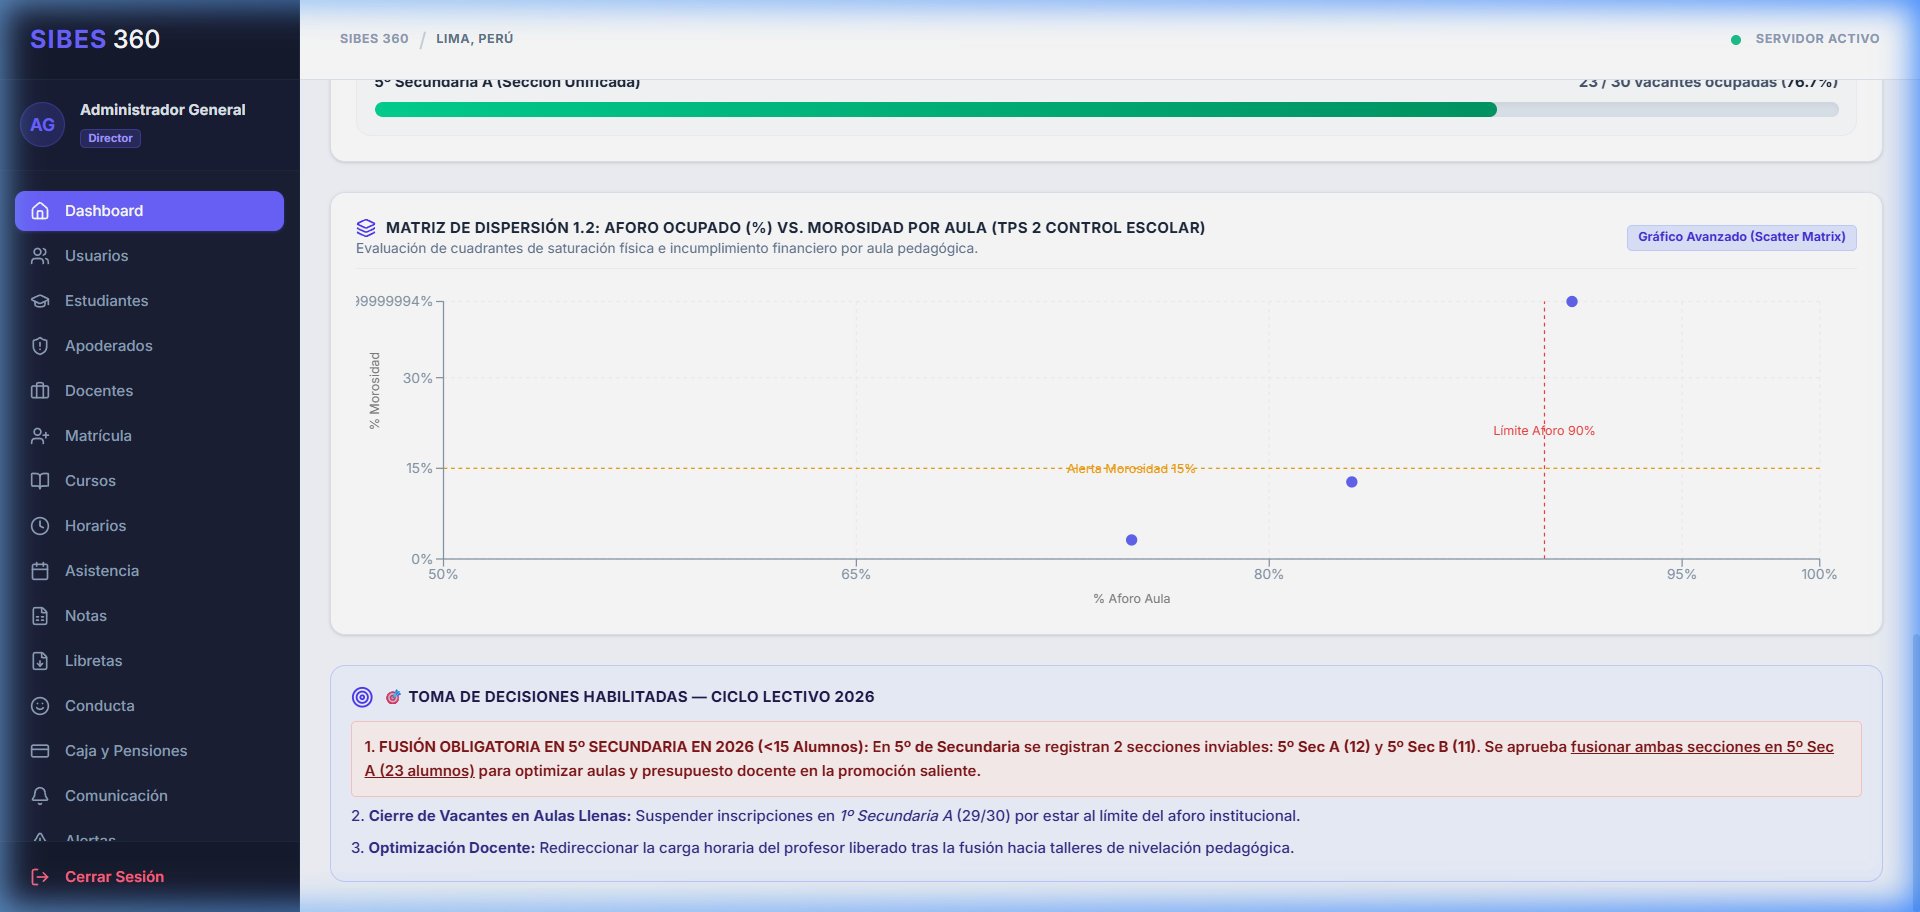
\includegraphics[width=0.95\textwidth]{tps2_control_escolar.png} 
        \caption{Dashboard Web Nativo TPS 2: Control de Matrículas, Aforo por Secciones y Matriz de Dispersión Aforo vs. Morosidad (Secretaría / Base de Datos Real)}
        \label{fig:dashboard_web_aforo}
    \end{figure}

    \begin{cajaConcepto}[Toma de Decisiones Operativas -- TPS 2 Control Escolar (Secretaría / Convivencia)]
    \textbf{Decisiones Inmediatas Habilitadas por la Base de Datos Real:}
    \begin{enumerate}
        \item \textbf{Cierre Automatizado por Saturación ($\text{TOV}_i \ge 95\%$):} Al constatar en tiempo real que 1º Secundaria "A" alcanzó 29/30 alumnos (96.7\%), el sistema cierra inscripciones en el aula y deriva nuevas vacantes hacia 1º "C" (22/30 vacantes).
        \item \textbf{Fusión Eficiente de Secciones Subocupadas ($<15$ Alumnos):} Reorganización de las aulas de 5º de Secundaria con baja matrícula (12 y 11 alumnos) en una única sección unificada de 23 estudiantes para optimizar costos docentes.
    \end{enumerate}
    \end{cajaConcepto}

    \section{Dashboard Operativo TPS 1: Rendimiento Académico y Evaluación CNEB (Subdirección Académica)}

    Desarrollado para la Dirección Académica y los docentes de asignatura:
    \begin{itemize}
        \item \textbf{Métricas de Calidad Pedagógica Real:} Evaluación Docente Promedio (\textbf{88.5\%}), Logro CNEB Alcanzado (\textbf{86.2\%}) y Tasa de Crecimiento Interanual de Matrícula (\textbf{CAGR +8.1\%}).
        \item \textbf{Gráfico Avanzado -- Radar Multidimensional de Calidad Escolar (4 Ejes):} Integra en un diagrama polar de 4 ejes el Rendimiento Académico CNEB ($86.2\%$), la Asistencia y Puntualidad ($94.8\%$), el Clima de Convivencia ($92.0\%$) y la Solvencia de Recaudación ($87.1\%$), comparando el año actual (2026) vs. el ciclo anterior (2025).
    \end{itemize}

    \begin{figure}[H]
        \centering
        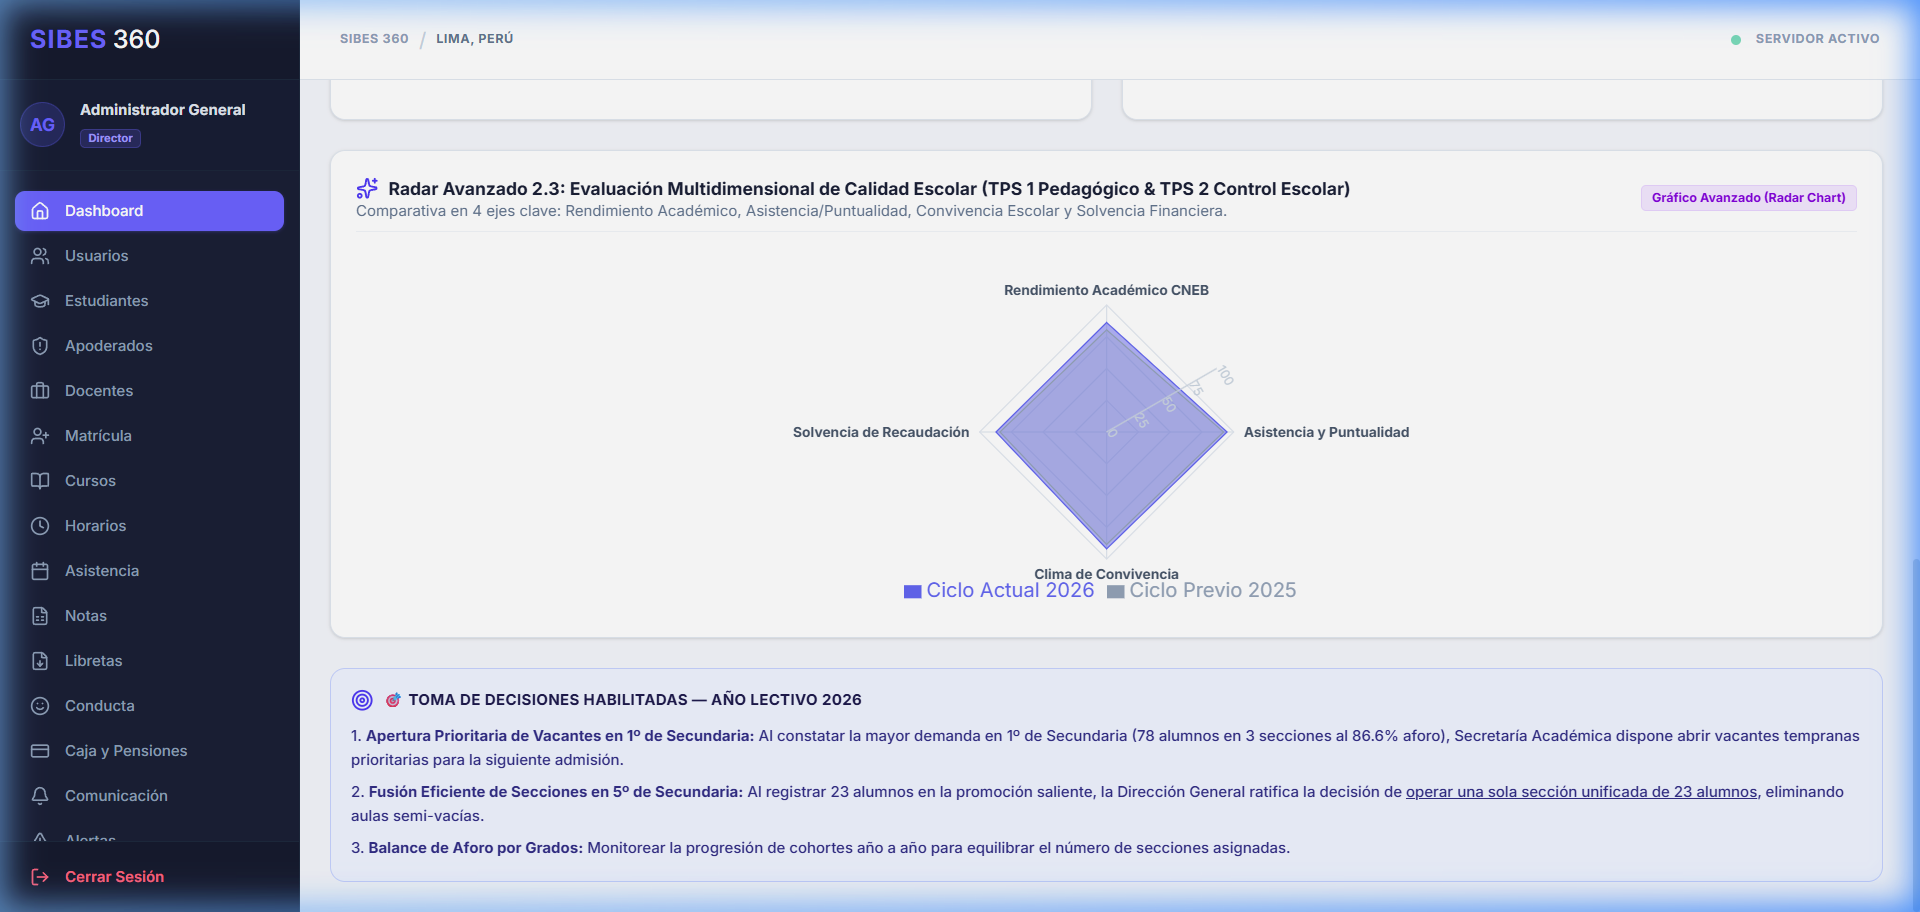
\includegraphics[width=0.95\textwidth]{tps1_pedagogico.png}
        \caption{Dashboard Web Nativo TPS 1: Rendimiento Académico, Evaluaciones por Competencias CNEB y Radar Multidimensional de Calidad (Dirección Académica)}
        \label{fig:dashboard_web_pedagogico}
    \end{figure}

    \begin{cajaConcepto}[Toma de Decisiones Operativas -- TPS 1 Pedagógico (Dirección Académica)]
    \textbf{Decisiones Inmediatas Habilitadas por la Base de Datos Real:}
    \begin{enumerate}
        \item \textbf{Intervención Pedagógica en Asignaturas de Alto Riesgo:} Reforzamiento académico para los 18 alumnos en escala C de Matemática y 14 alumnos en Física-Química.
        \item \textbf{Ajuste del Plan Docente Bimestral:} Nivelación obligatoria en 3º de Secundaria tras registrar un promedio ponderado de 14.5.
    \end{enumerate}
    \end{cajaConcepto}

    \section{Matriz 2x2 de Interacción Transaccional Directa: TPS 1 (Pedagógico) $\leftrightarrow$ TPS 2 (Control Escolar)}

    Esta pantalla principal ilustra la integración directa entre los dos sistemas de procesamiento de transacciones (\textbf{TPS 1 Pedagógico} y \textbf{TPS 2 Control Escolar}) mediante una matriz de \textbf{4 gráficos analítico-transaccionales dispuesta en 2 filas y 2 columnas}:

    \begin{itemize}
        \item \textbf{Gráfico 1 (Fila 1, Columna 1 -- Asistencia vs. Rendimiento):} Cruza el porcentaje de asistencia registrado en puerta por Auxiliaría (\textbf{TPS 2}) con la nota promedio bimestral y la tasa de reprobación en la escala CNEB (\textbf{TPS 1}). Demuestra que el ausentismo escolar ($<90\%$) cuadruplica el riesgo de reprobación ($28.4\%$).
        \item \textbf{Gráfico 2 (Fila 1, Columna 2 -- Conducta vs. Rendimiento):} Relaciona las incidencias disciplinarias de la bitácora de convivencia (\textbf{TPS 2}) con el rendimiento académico CNEB (\textbf{TPS 1}), revelando que los alumnos con faltas graves sufren una caída en su promedio de $16.8$ a $11.8$.
        \item \textbf{Gráfico 3 (Fila 2, Columna 1 -- Ausentismo en Cursos Críticos):} Desglosa la cantidad de estudiantes desaprobados en nivel C de Matemática (18 alumnos) y Física-Química (14 alumnos) que acumulan inasistencias en el primer bloque lectivo.
        \item \textbf{Gráfico 4 (Fila 2, Columna 2 -- Trigger SQL de Reprogramación):} Monitorea la ejecución en tiempo real del Trigger SQL \texttt{trg\_aprobar\_justificacion\_evaluacion}, el cual, tras la aprobación de una falta médica en Secretaría (\textbf{TPS 2}), habilita atómicamente la reprogramación de exámenes en el registro docente (\textbf{TPS 1}).
    \end{itemize}

    \begin{figure}[H]
        \centering
        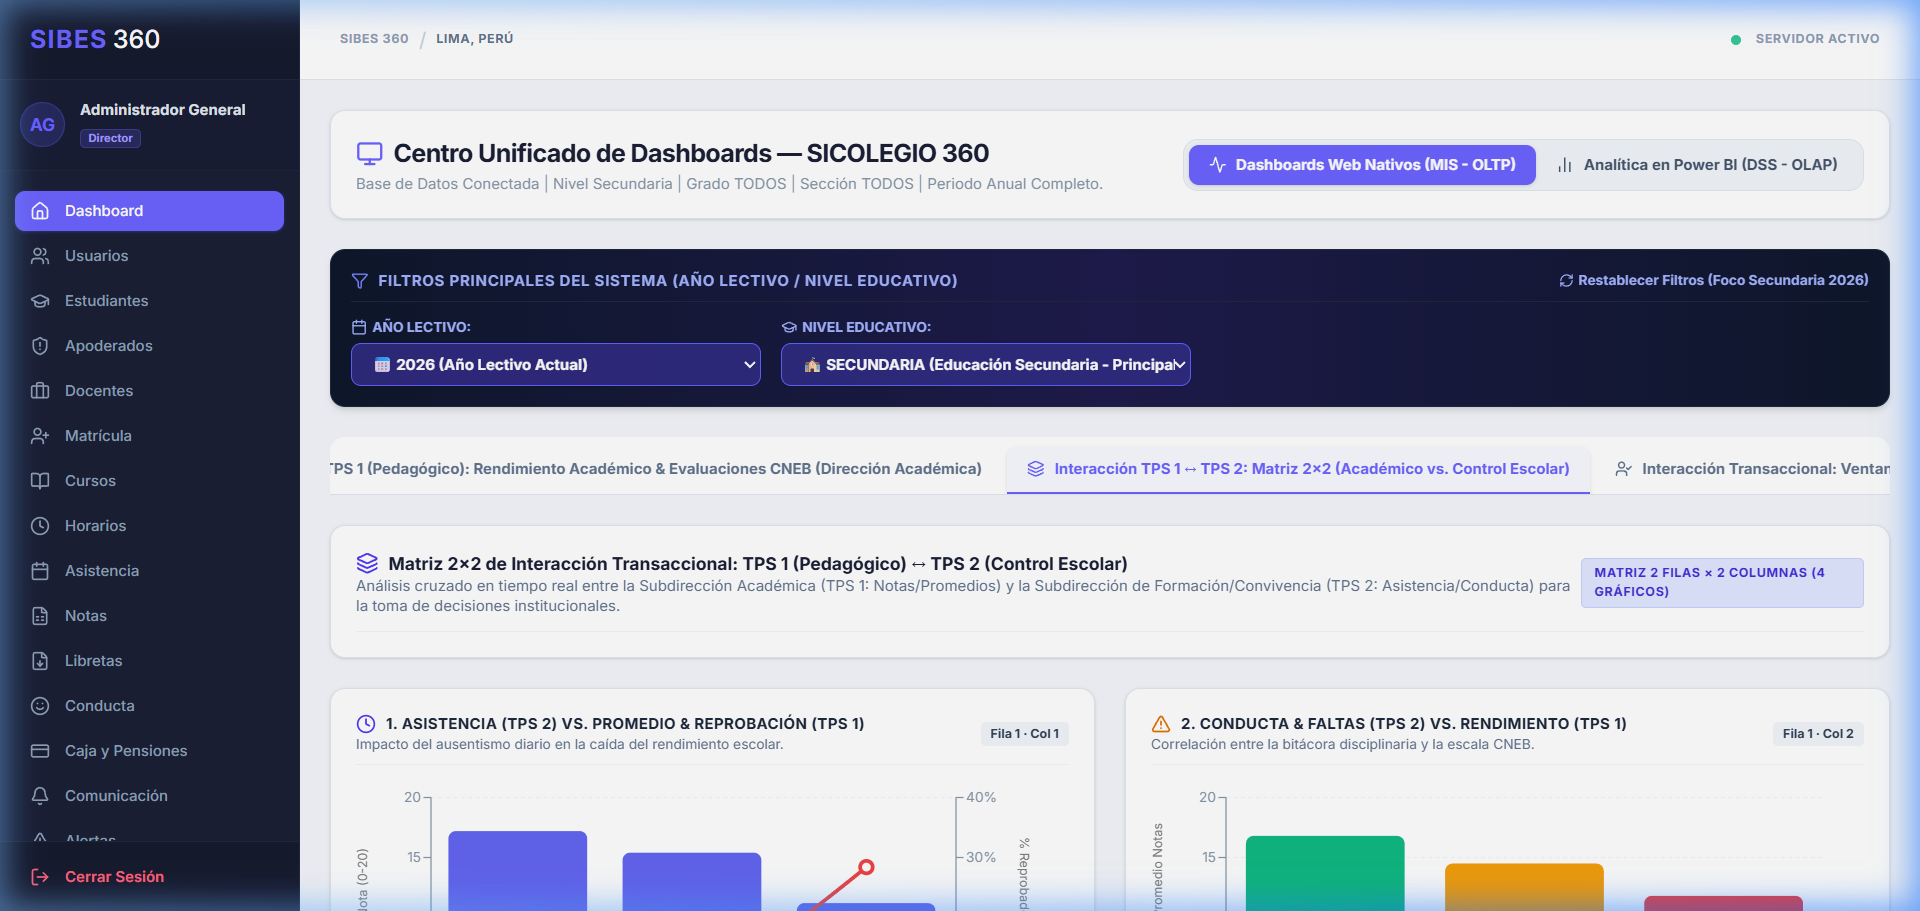
\includegraphics[width=0.98\textwidth]{tps_interaccion_2x2.png}
        \caption{Matriz 2x2 de Interacción Transaccional: TPS 1 (Pedagógico) $\leftrightarrow$ TPS 2 (Control Escolar) con 4 Gráficos Dispuestos en 2 Filas y 2 Columnas}
        \label{fig:tps_interaccion_2x2}
    \end{figure}

    \begin{cajaConcepto}[Toma de Decisiones Operativas -- Matriz 2x2 Interacción TPS 1 $\leftrightarrow$ TPS 2]
    \textbf{Decisiones Inter-áreas Habilitadas por la Base de Datos Real:}
    \begin{enumerate}
        \item \textbf{Intervención Conjunta por Ausentismo Crónico:} Secretaría y Dirección Académica citan al apoderado cuando la asistencia cae por debajo del 90\%, suscribiendo compromisos de puntualidad y asignando tutorías remediantes antes del cierre bimestral.
        \item \textbf{Derivación al Programa Psicopedagógico de Convivencia:} Orientación obligatoria para estudiantes con acumulación de deméritos en TPS 2 para mitigar el deterioro académico en TPS 1.
        \item \textbf{Garantía Transaccional Zero-Errors (Trigger SQL):} Eliminación del riesgo de asignación indebida de nota "00" a alumnos con ausencias justificadas legalmente por Secretaría.
    \end{enumerate}
    \end{cajaConcepto}

    \section{Dashboard Operativo TPS 3: Ventanilla Única y Expediente 360 del Estudiante (Tesorería / Administración)}

    Permite atender al apoderado en ventanilla de forma integrada:
    \begin{itemize}
        \item \textbf{Expediente 360º en Tiempo Real:} Consulta unificada por DNI (ej. Mateo Andrés Quispe Morales, DNI: 74829103) combinando datos académicos, récords de asistencia y compromisos financieros en una sola pantalla.
    \end{itemize}

    \begin{figure}[H]
        \centering
        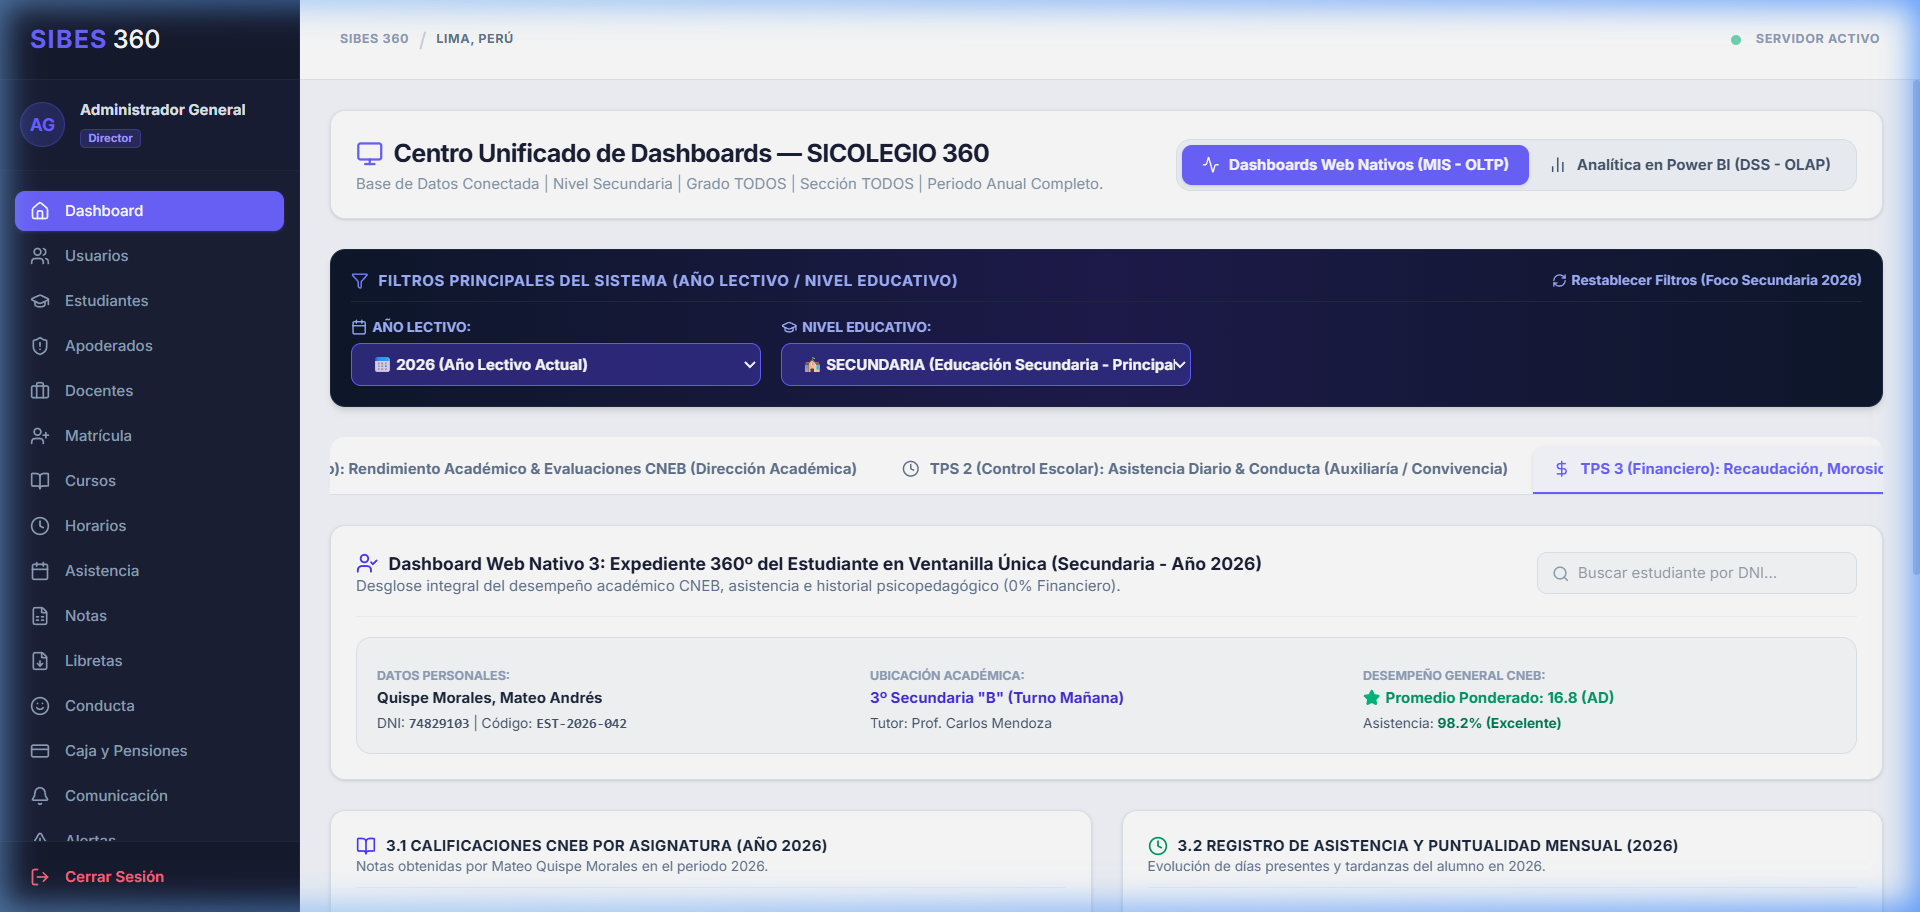
\includegraphics[width=0.95\textwidth]{tps3_financiero.png}
        \caption{Dashboard Web Nativo TPS 3: Expediente 360º del Estudiante en Ventanilla Única (Tesorería / Administración)}
        \label{fig:dashboard_web_ficha}
    \end{figure}

    \begin{cajaConcepto}[Toma de Decisiones Operativas -- TPS 3 Ventanilla Única (Tesorería / Administración)]
    \textbf{Decisiones Inmediatas Habilitadas por la Base de Datos Real:}
    \begin{enumerate}
        \item \textbf{Emisión Automatizada de Libretas y Solvencias:} Emisión directa de libretas escolares y constancias al verificar el estado de pago al día.
        \item \textbf{Arqueo y Conciliación de Caja Operativa (TPS-11):} Cuadre inmediato de cobranzas por pasarela web, tarjetas POS y efectivo.
    \end{enumerate}
    \end{cajaConcepto}

    % ═══════════════════════════════════════════════════════════════
    %  CAPÍTULO V: MODELADO E INTEGRACIÓN ANALÍTICA EN POWER BI (DSS)
    % ═══════════════════════════════════════════════════════════════
    \chapter{Modelado e Integración Analítica en Power BI (Nivel DSS / BI Estratégico)}

    \section{Del Modelo Transaccional (OLTP) al Modelo Analítico (OLAP)}

    Mientras que los dashboards web nativos del Capítulo III le sirven al secretario y tesorero para operar la jornada diaria, la Promotora y la Dirección General requieren una perspectiva \textbf{analítica, histórica y multidimensional}. Realizar consultas de agregación masiva (\texttt{SUM}, \texttt{AVG}, \texttt{GROUP BY}) sobre la base de datos relacional OLTP degradaría el rendimiento de las transacciones operativas de la escuela.

    Por esta razón, SICOLEGIO 360 implementa un pipeline analítico que extrae los datos de la base centralizada mediante \textbf{Vistas SQL especializadas (Capa ETL)} y los carga en el motor analítico \textit{VertiPaq} de \textbf{Microsoft Power BI}, transformando la estructura relacional en un \textbf{Modelo Dimensional en Estrella (\textit{Star Schema})}.

    \section{Pipeline ETL y Vistas SQL de Extracción}

    Para alimentar a Power BI sin exponer las tablas crudas del sistema, se crean vistas SQL optimizadas en la base de datos centralizada. El Anexo A incluye los scripts DDL de estas vistas. La vista principal \texttt{vw\_FactMatriculaPagos} desnormaliza los eventos financieros y académicos:

    \begin{lstlisting}[language=SQL, caption={Vista SQL de extracción ETL para la Tabla de Hechos en Power BI}]
    CREATE VIEW vw_FactMatriculaPagos AS
    \section{Pipeline ETL y Vistas SQL de Extracción}

    Para alimentar a Power BI sin exponer las tablas crudas del sistema, se crean vistas SQL optimizadas en la base de datos. La vista principal \texttt{vw\_FactRendimientoAsistencia} desnormaliza los eventos académicos y el registro de control escolar:

    \begin{lstlisting}[language=SQL, caption={Vista SQL de extracción ETL para la Tabla de Hechos en Power BI}]
    CREATE VIEW vw_FactRendimientoAsistencia AS
    SELECT 
        n.id_nota AS id_hecho_evaluacion,
        m.id_estudiante,
        m.id_seccion,
        n.id_curso,
        CAST(DATE_FORMAT(n.fecha_registro, '%Y%m%d') AS UNSIGNED) AS id_fecha_evaluacion,
        n.calificacion_numerica AS nota_obtenida,
        CASE WHEN n.calificacion_numerica < 11 THEN 1 ELSE 0 END AS es_desaprobado,
        COALESCE(a.total_asistencias, 0) AS total_asistencias,
        COALESCE(a.total_inasistencias, 0) AS total_inasistencias,
        COALESCE(c.demeritos_acumulados, 0) AS demeritos_conducta
    FROM notas n
    INNER JOIN matriculas m ON n.id_estudiante = m.id_estudiante
    LEFT JOIN (
        SELECT id_estudiante, 
            SUM(CASE WHEN estado = 'PRESENTE' THEN 1 ELSE 0 END) AS total_asistencias,
            SUM(CASE WHEN estado = 'FALTA' THEN 1 ELSE 0 END) AS total_inasistencias
        FROM asistencias GROUP BY id_estudiante
    ) a ON m.id_estudiante = a.id_estudiante
    LEFT JOIN (
        SELECT id_estudiante, SUM(puntos_demerito) AS demeritos_acumulados
        FROM conducta GROUP BY id_estudiante
    ) c ON m.id_estudiante = c.id_estudiante;
    \end{lstlisting}

    \section{Modelado Dimensional en Estrella (Star Schema)}

    El modelo de datos analítico dentro de Power BI está diseñado en un \textbf{Esquema en Estrella} clásico alrededor de la tabla de hechos central \texttt{FactRendimientoAsistencia}, conectada a cuatro dimensiones mediante relaciones de uno a muchos ($1:*$):

    \begin{figure}[H]
        \centering
        \begin{cajaConcepto}[Esquema en Estrella de Power BI -- SICOLEGIO 360]
        \textbf{Tabla de Hechos (Fact Table):}
        \begin{itemize}
            \item \texttt{FactRendimientoAsistencia} (\textit{nota\_obtenida, es\_desaprobado, total\_asistencias, total\_inasistencias, demeritos\_conducta})
        \end{itemize}
        \textbf{Tablas de Dimensiones (Dimension Tables):}
        \begin{itemize}
            \item \texttt{DimEstudiante} (\textit{id\_estudiante, dni, nombre\_completo, estado\_academico, grado, seccion})
            \item \texttt{DimCurso} (\textit{id\_curso, nombre\_curso, area\_curricular, horas\_semanales})
            \item \texttt{DimSeccion} (\textit{id\_seccion, nombre\_seccion, aforo\_maximo, tutor\_asignado})
            \item \texttt{DimTiempo} (\textit{id\_fecha, fecha, anio, mes, bimestre, trimestre})
        \end{itemize}
        \end{cajaConcepto}
        \caption{Modelado dimensional en estrella diseñado para Power BI}
        \label{fig:star_schema}
    \end{figure}

    \section{Desarrollo de Expresiones DAX para KPIs Estratégicos}

    En Power BI, la inteligencia de negocios se construye mediante fórmulas en lenguaje \textbf{DAX (\textit{Data Analysis Expressions})}. A continuación se presentan las medidas clave implementadas para la gestión de SICOLEGIO 360:

    \paragraph{1. Promedio General de Rendimiento Académico:}
    \begin{lstlisting}
    PromedioGeneralRendimiento = AVERAGE(FactRendimientoAsistencia[nota_obtenida])
    \end{lstlisting}

    \paragraph{2. Porcentaje de Desaprobación por Asignatura:}
    \begin{lstlisting}
    % Desaprobacion = 
    VAR TotalEvaluados = COUNT(FactRendimientoAsistencia[id_hecho_evaluacion])
    VAR TotalDesaprobados = SUM(FactRendimientoAsistencia[es_desaprobado])
    RETURN
    DIVIDE(TotalDesaprobados, TotalEvaluados, 0)
    \end{lstlisting}

    \paragraph{3. Tasa de Asistencia Ponderada:}
    \begin{lstlisting}
    TasaAsistenciaPonderada = 
    VAR TotalAsist = SUM(FactRendimientoAsistencia[total_asistencias])
    VAR TotalFaltas = SUM(FactRendimientoAsistencia[total_inasistencias])
    RETURN
    DIVIDE(TotalAsist, TotalAsist + TotalFaltas, 0)
    \end{lstlisting}

    \paragraph{4. Índice Promedio de Incidencias de Conducta:}
    \begin{lstlisting}
    IndiceDemeritosConducta = 
    AVERAGE(FactRendimientoAsistencia[demeritos_conducta])
    \end{lstlisting}

    \section{Dashboards Estratégicos en Power BI para la Alta Dirección}

    Con el modelo dimensional y las medidas DAX construidas, se desarrollan cuatro paneles de control gerenciales dentro del informe de Power BI:

    \subsection{Dashboard Power BI 1: Radar de Rendimiento Académico y Desaprobación por Grado}

    \end{document}
